\lysh{15176}{2}
\begin{alist}
\item Είναι $P(1) = 1^3 - 2 \cdot 1^2 + 3 \cdot 1 - 2 = 0$, άρα το 1 είναι μία ρίζα του πολυωνύμου. \\
Επιπλέον ισχύει ότι
\[1 \text{ ρίζα του } P(x) \Leftrightarrow x - 1 \text{ παράγοντας του } P(x)\]
\item Είναι: $P(x) = (x - 1)(x^2 - x + 2)$. \\
Το τριώνυμο $x^2 - x + 2 \ne 0$ διότι έχει διακρίνουσα αρνητική και επιπρόσθετα ισχύει ότι $x^2 - x + 2 > 0$ για κάθε $x \in \mathbb{R}$. \\
Άρα $P(x) = 0 \Leftrightarrow (x - 1)(x^2 - x + 2) = 0 \Leftrightarrow x = 1$. \\
Το πρόσημο των τιμών του $P(x)$ φαίνεται στον παρακάτω πίνακα προσήμων:
\begin{center}
\begin{tikzpicture}
\tkzTabInit[color,lgt=3,espcl=2,colorC = maincolor!40,
colorL = maincolor!20,
colorV = maincolor!40]%
  {$x$ /1, $x-1$ /1, $x^2-x+2$ /1, $P(x)$ /1}
  {$-\infty$, $1$, $+\infty$}
\tkzTabLine{ , -, z, +, }
\tkzTabLine{ , +, d, +, }
\tkzTabLine{ , -, z, +, }
\end{tikzpicture}
\end{center}
Ως εκ τούτου, είναι: $P(x) > 0 \Leftrightarrow x > 1$.
\end{alist}

